\subsection{Installazione}

Prima di poter installare l'applicazione è necessario attivare l'opzione "Origini sconosciute" nelle impostazioni.
Per attivare tale opzione è necessario:
\begin{itemize}
	\item andare in Impostazioni
	\item selezionare Sicurezza
	\item attivare "Origini sconosciute"
\end{itemize}

\begin{figure}[!h]
	\centering
	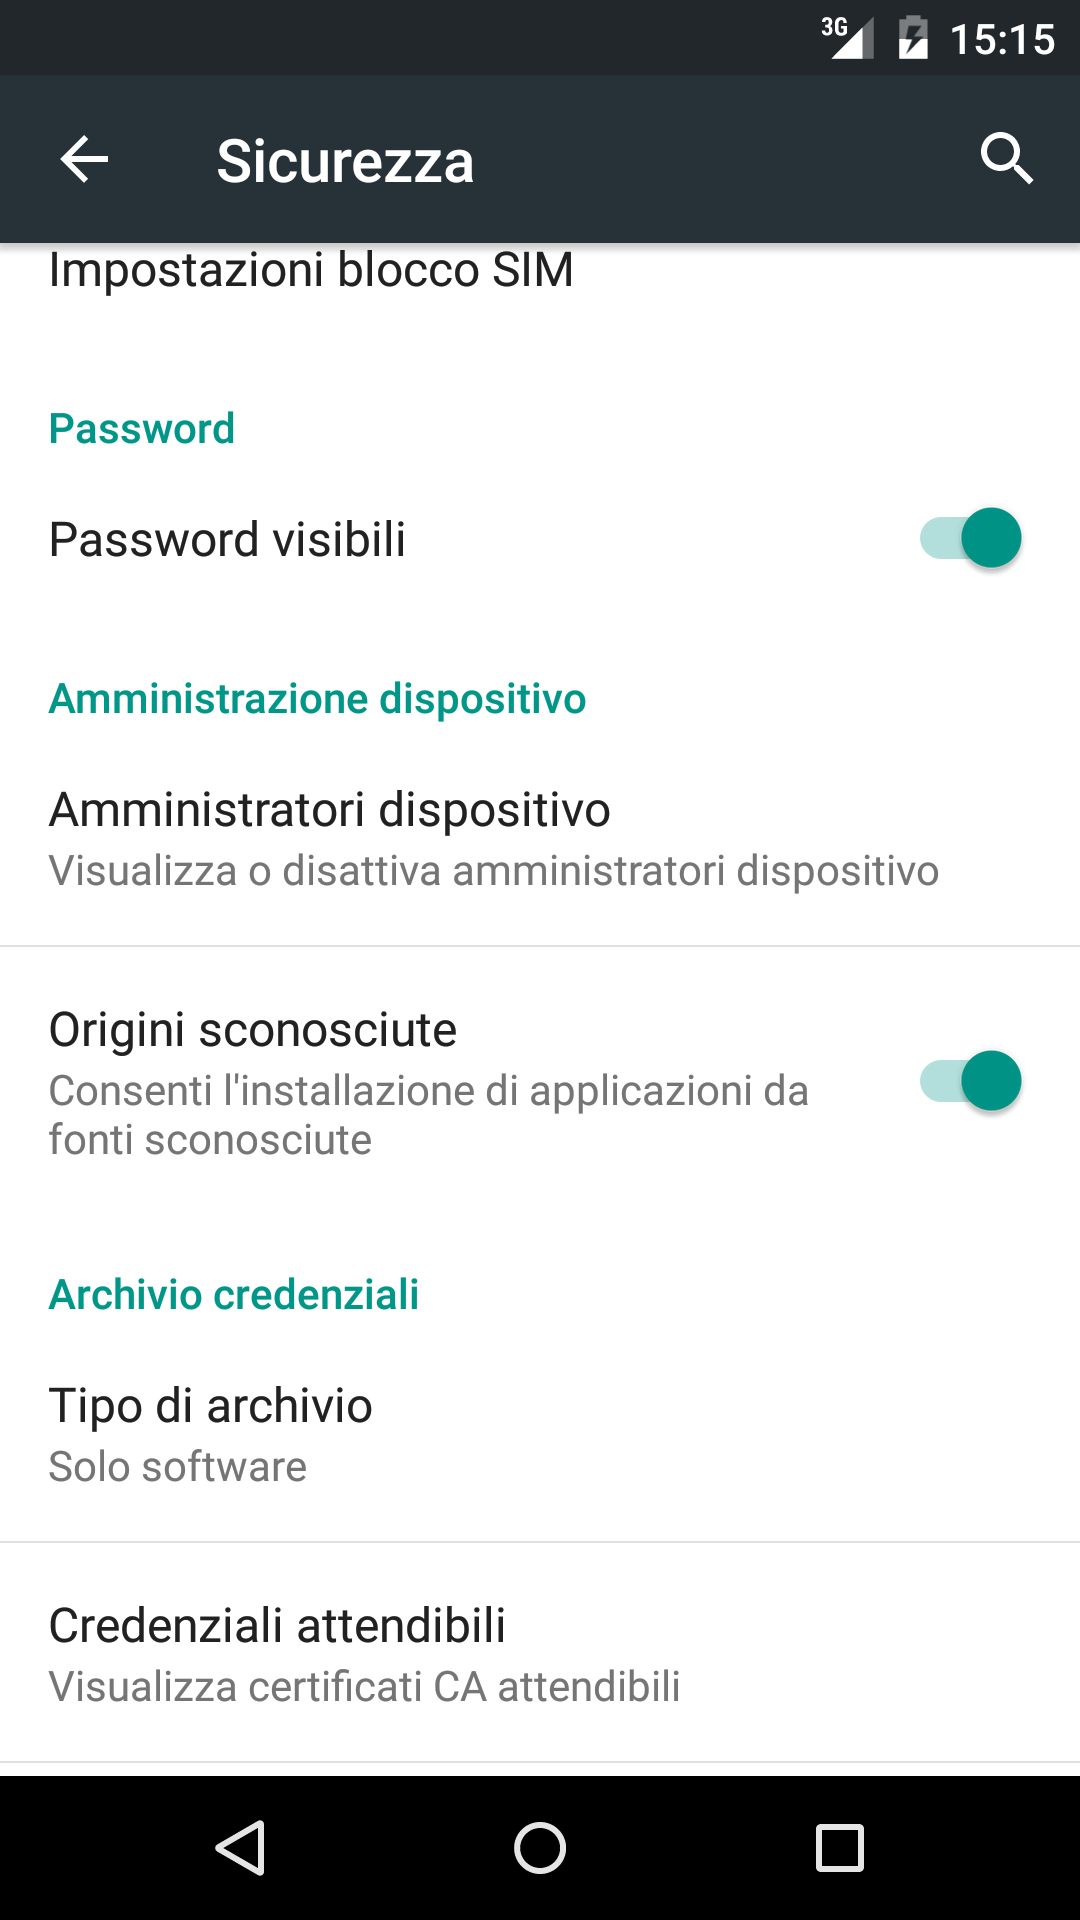
\includegraphics[scale=0.10]{screenshot/origini_sconosciute}
	\caption{Schermata opzione Origini Sconosciute}
\end{figure}

Una volta che ci si è assicurati di avere l'opzione "Origini sconosciute" attiva è necessario visitare il sito \url{http://beaconstrips.tk} e premere sul tasto "Download" che si trova verso il fondo della pagina.

\begin{figure}[!h]
	\centering
	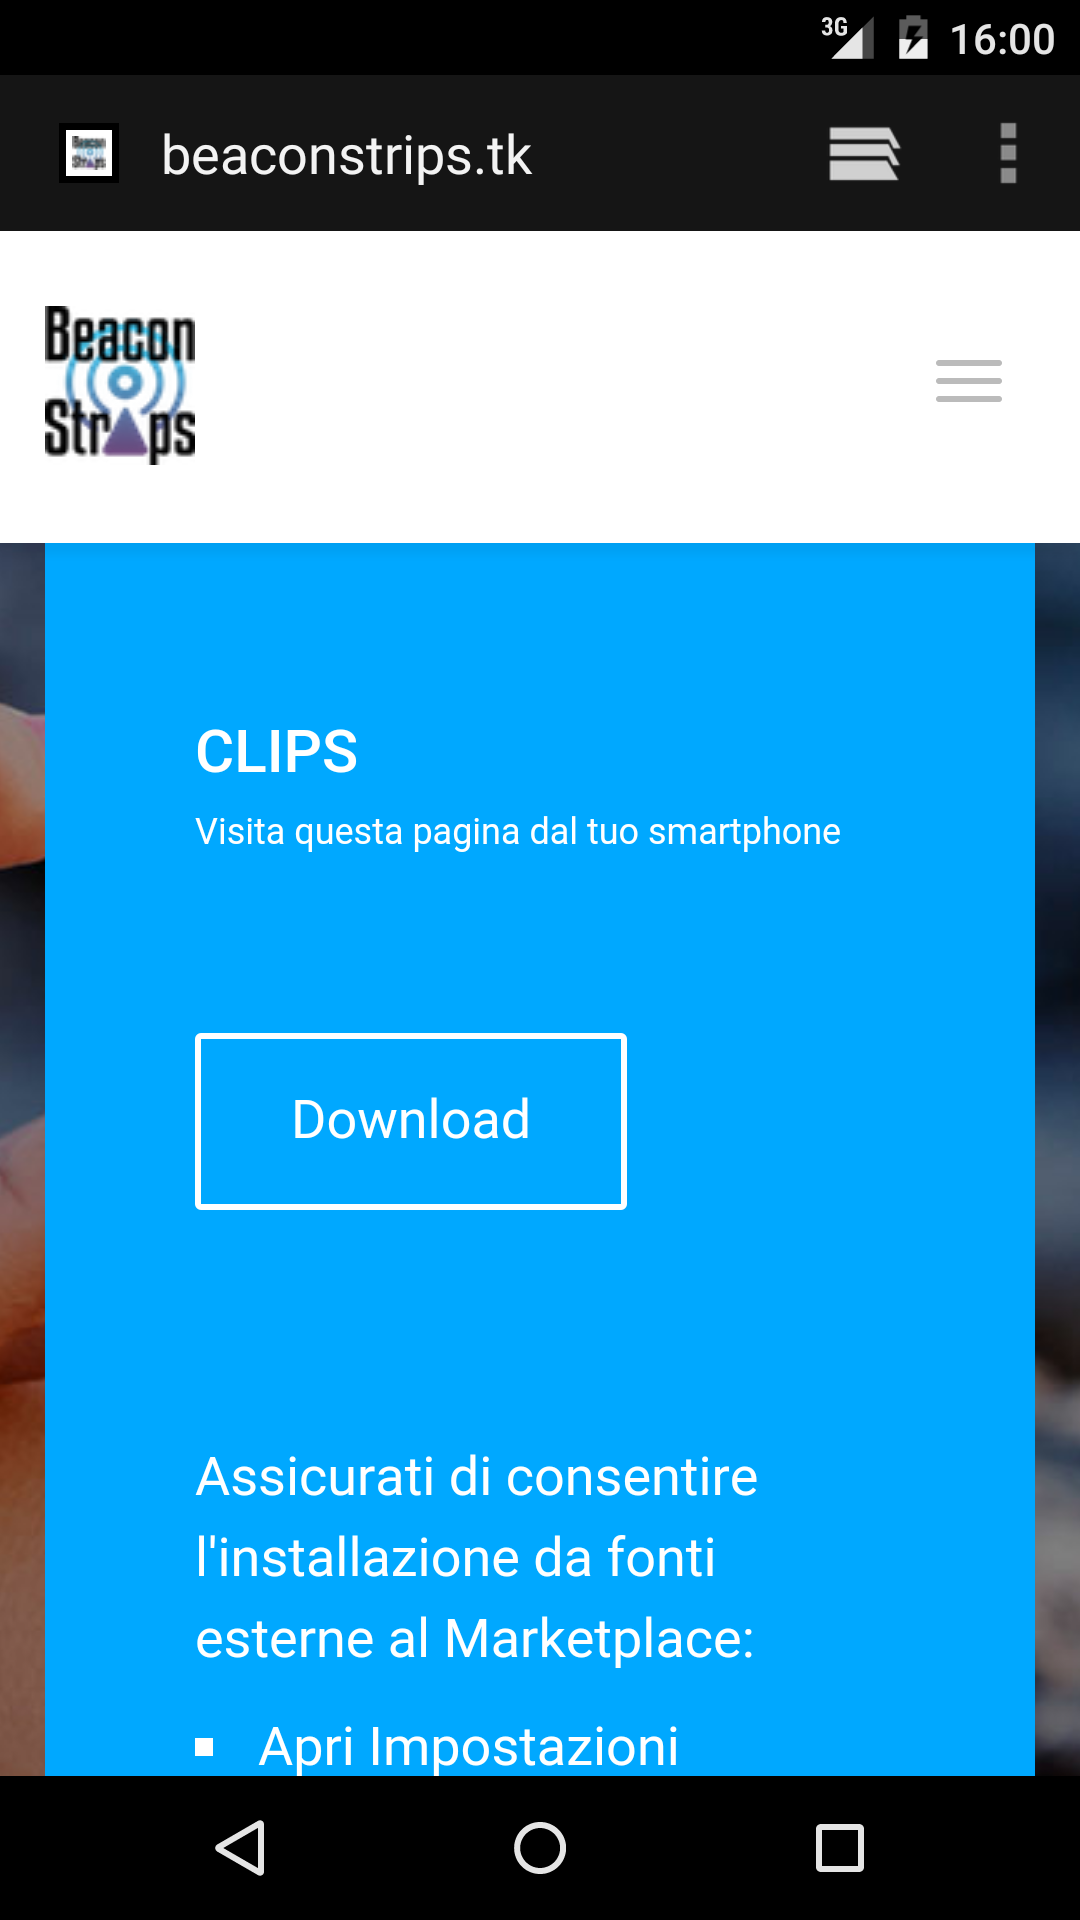
\includegraphics[scale=0.10]{screenshot/download}
	\caption{Schermata di download}
\end{figure}

Una volta scaricato il file è necessario premere sulla notifica del completamento del download per far partire il processo di installazione. Infine seguire le istruizioni a schermo per completare il processo.

\begin{figure}[!h]
	\centering
	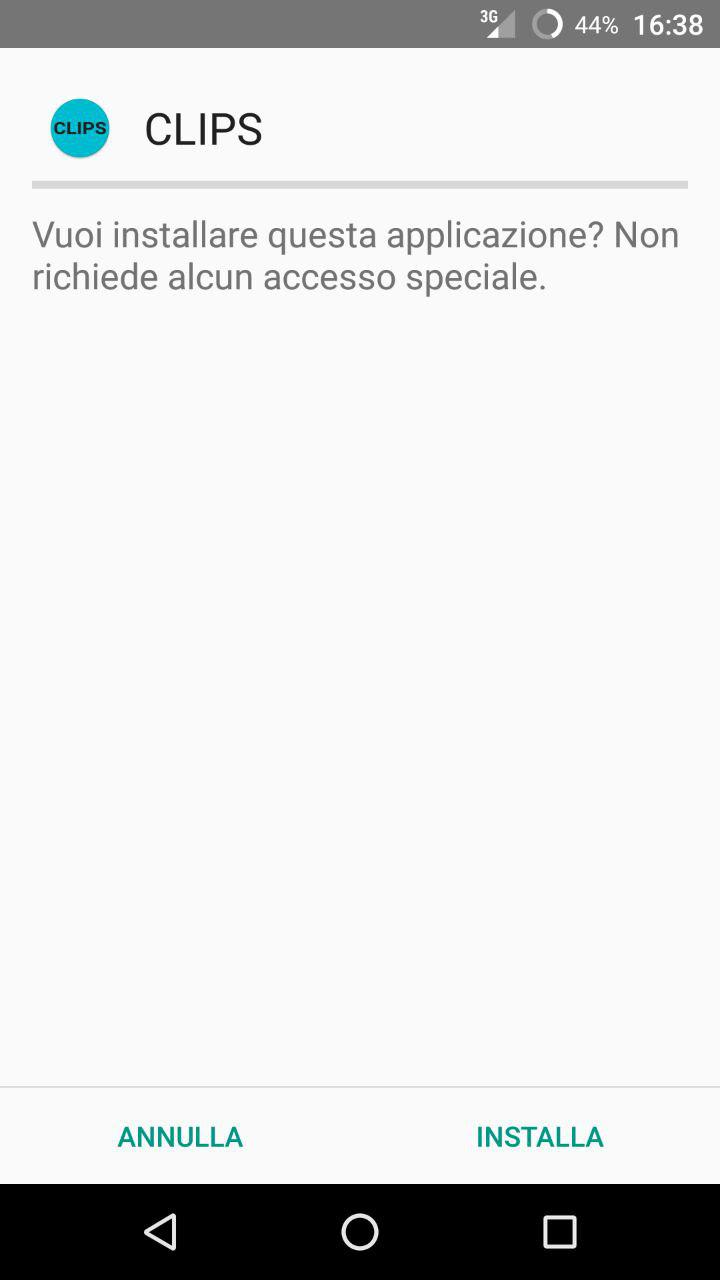
\includegraphics[scale=0.15]{screenshot/installa}
	\caption{Schermata di installazione}
\end{figure}

\subsubsection{Aggiornamento}

Per aggiornare l'applicazione è sufficiente seguire i passi precedentemente descritti. Una volta premuto sulla notifica del completamento del download vi verrà chiesto se volete aggiornare l'applicazione. Premere sì e proseguire con le istruzioni a schermo per completare il processo.

\begin{figure}[!h]
	\centering
	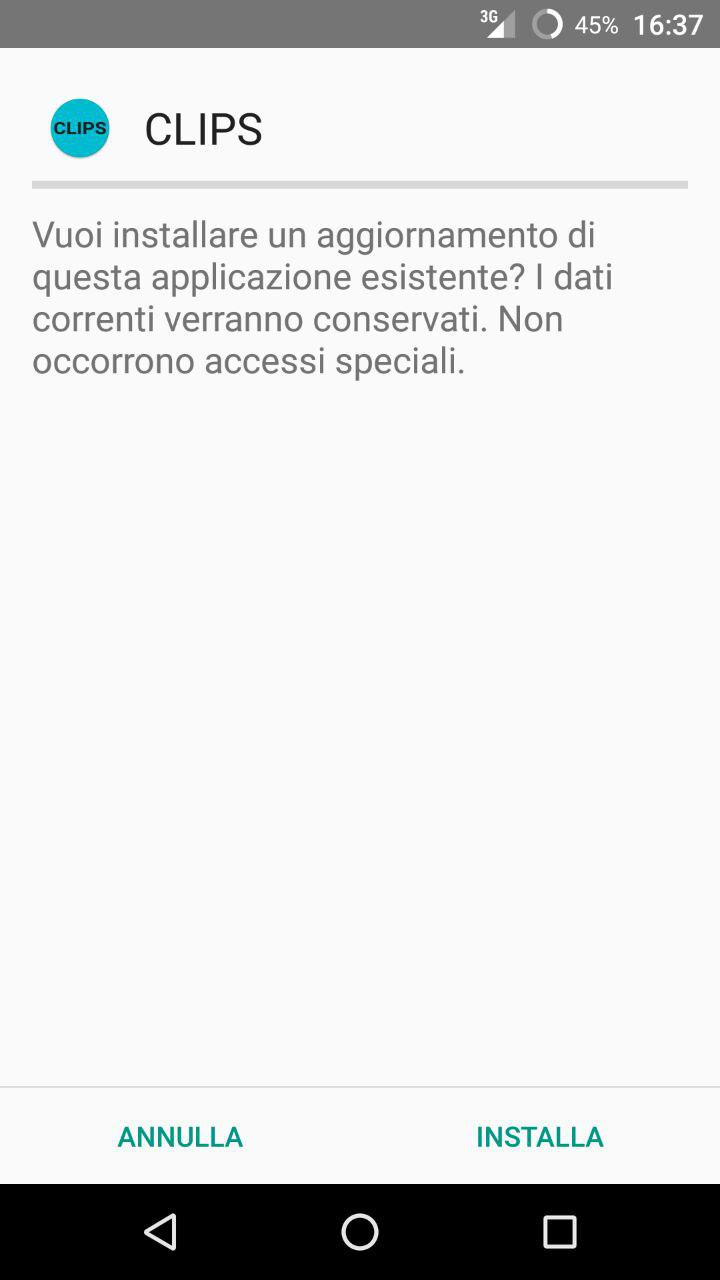
\includegraphics[scale=0.15]{screenshot/aggiorna}
	\caption{Schermata di aggiornamento}
\end{figure}